\section{Gait Recognition-based Physical Access Control}
\label{sec:gait-recognition-for-physical-access-control}

\subsection{Gait Recognition Overview}
\label{subsec:gait-recognition-overview}

\ac{gr} technology assesses a combination of biometric information to determine identity based on walking patterns.
Both physiological (e.g., body shape) and behavioural (e.g., walking speed) attributes can contribute, with data typically collected using \ac{cv} techniques \cite{mallickFastGaitRecognition2016}, or in some cases, under-floor pressure sensors \parencite{stepscanGaitAuthenticationSecurity2020}.

As discussed in Section \ref{subsec:biometric-authentication-trends}, biometric identification is enabled by analysing features derived from biological data (e.g., face shape and nose position for face recognition).
Gait-related features can be statistical, or spatiotemporal.
Statistical features describe attributes over time, like average stride length and speed, and their standard deviation and variability, whereas spatiotemporal features describe a subject's movement over a defined area and (time) period.
Gait analysis often uses a combination of statistical and spatiotemporal information, with assessment of an entire movement cycle typically necessitating both \parencite{gunersahanSurveyAppearancebasedApproaches2024}.

The level of security enabled by common biometric authentication techniques (see Section \ref{subsec:biometric-authentication-trends}) could be maintained by \ac{gr} --- analysing hard-to-replicate, difficult-to-disguise inherence factors \parencite{nevesChapter1Unconstrained2017a}.
By assessing body movement to determine identity, \ac{gr} can work from a distance without user participation, contributing to what this project aims to achieve.
Unlike facial recognition, \ac{gr} is impacted less by lower sensor resolutions (many appearance-based solutions, see \ref{subsubsec:appearance-based-approaches}, use low-resolution silhouette images) and face coverings --- benefiting reliability \parencite{cooperEffectsFaceCoverings2022}.
However, occlusion of other body parts may still have a performance impact (especially for \ac{cv}-based implementations).

There are not many examples of real-world \ac{pacs}s using \ac{gr} for authentication despite the moderate amount of \ac{cv}-based \ac{gr} research that exists.
\ac{cv}-based \ac{gr} has seen clinical use, however, where gait has been assessed to treat stroke victims and Cerebral Palsy \parencite{davisReflectionsClinicalGait1997}.
Law enforcement have also demonstrated how \ac{gr} can be used to asynchronously identify criminals from \ac{cctv} footage \parencite{nebulampKannurPoliceFollow2024}.
These examples prove a significant amount of information can be discerned from gait, but do so outside \ac{pacs} constraints, within which there is a target for how long identification takes to ensure users can be promptly granted access \parencite{sandhuAccessControlPrinciple1994}.
\textit{This project applies techniques like the above in a real-time context to achieve hands-free user authentication for use in a \ac{pacs}, performing identification based on movement information captured from a live video feed.}

A rare real-world example of \ac{gr} being used for authentication is 'Stepscan Secure' --- a product described as the 'world's first pressure-based gait-authentication system for access control'.
It uses under-floor pressure sensors to assess walking patterns \parencite{stepscanGaitAuthenticationSecurity2020}.
While pricing information is not publicly available (and \citeauthor{stepscanGaitAuthenticationSecurity2020} did not respond to queries), the assumption can be made that the cost of implementation would be higher than a \ac{cv}-based solution that uses just a camera.
This is because enough pressure sensors must be purchased to span an entrance way, which would also increase costs as the operational distance requirements grow, compared to a \ac{cv}-based approach which would inherently work at further distances, restricted by only what camera resolution allows.

In reference to the ethical topics discussed in \ref{subsec:biometric-authentication-trends}:
bias concerns also apply to \ac{gr}, but unlike facial recognition, relate more to sex and age, calling for on diversity in body shape for datasets (especially in \ac{cv}-based \ac{gr}) and not necessarily in skin tone.
The CASIA-B dataset (124 subjects captured from 11 angles) is widely used for benchmarking in \ac{gr} research, but does not specify details about, nor appear to target diversity. However it does visibly include a split between male and female subjects \parencite{fuCASIABPoseCASIABPose2023}.
Comparatively, the OU-ISIR Large Population Dataset, is advertised to contain subjects aged 'ranging from 1 to 94 years' and a balanced gender distribution \parencite{iwamaOUISIRGaitDatabase2012}.

The following sections assess different \ac{cv}-based \ac{gr} techniques, each of which can be used to identify and authenticate individuals effectively by \ac{pacs}.

\subsection{Computer Vision-based Gait Recognition Techniques}
\label{subsec:cv-based-gr-techniques}

\subsubsection{Model-based Approaches}
\label{subsubsec:model-based-approaches}

Model-based \ac{gr} systems are a \ac{cv}-based approach that use attributes extracted from 2 or 3-dimensional 'models' to determine identity.
These models, often 'skeleton'-based (collections of joint positions) can be constructed using open-source libraries like 'OpenPose', which analyse footage and 'detect human body, hand, facial, and foot key points'.
Figure \ref{fig:openpose-pose-estimation} shows (a) an RGB image given as input to OpenPose and (b) the output 2D pose prediction \parencite{caoOpenPoseRealtimeMultiPerson2019}.
Purpose-made hardware like Microsoft's 'Kinect' sensors is also capable of capturing joint information in real-time, this can be used to construct similar models or for analysing the statistical data (e.g., in \ac{json} format).
Model-based data enables features like pose, limb lengths, and joint angles to be extracted, contributing to \ac{ml} classification efforts for person identification \parencite{liaoModelbasedGaitRecognition2020}.

\begin{figure}[H]
    \centering
    \begin{minipage}{0.48\textwidth}
        \centering
        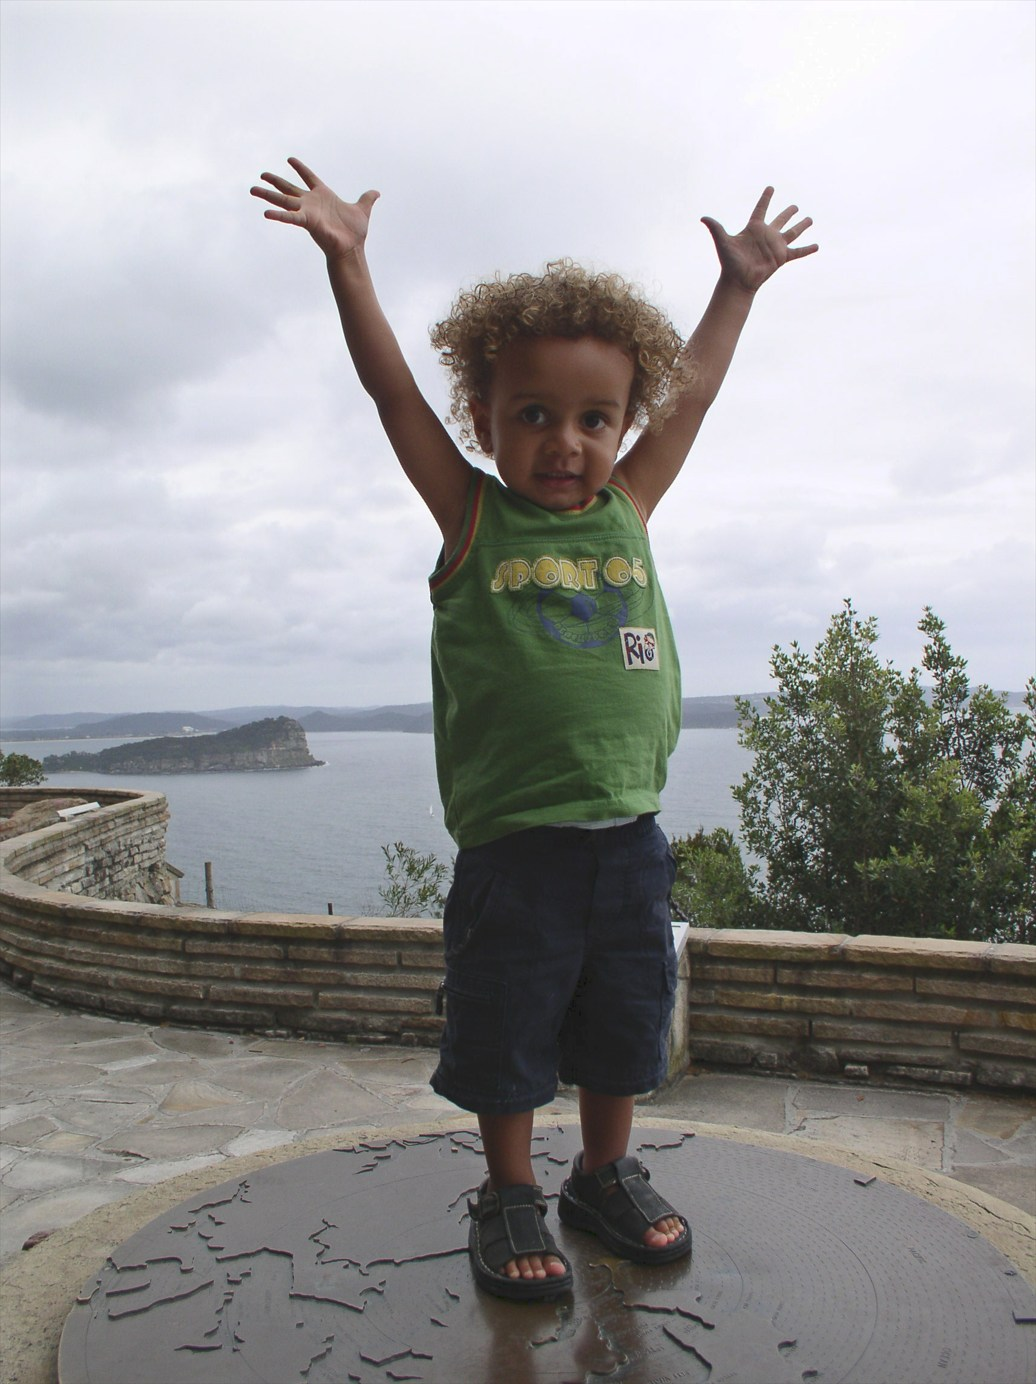
\includegraphics[width=\linewidth]{assets/raff-source.jpg}
        \subcaption{RGB Source Image}
        \label{fig:openpose-pose-estimation_a}
    \end{minipage}
    \hfill
    \begin{minipage}{0.48\textwidth}
        \centering
        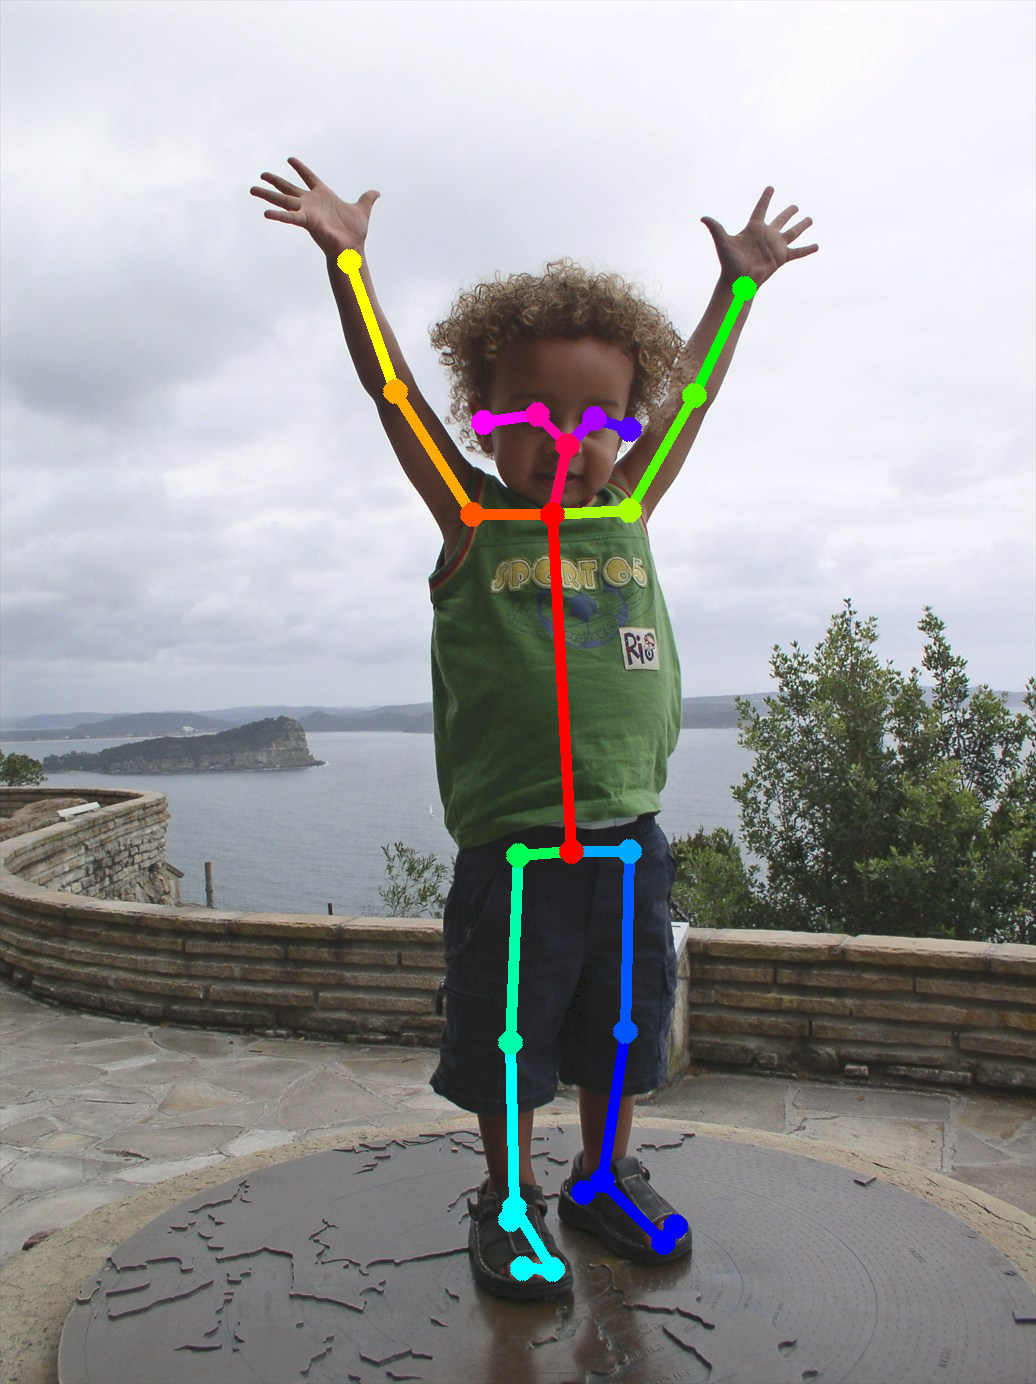
\includegraphics[width=\linewidth]{assets/raff-source_rendered.png}
        \subcaption{Pose Estimation with OpenPose}
        \label{fig:openpose-pose-estimation_b}
    \end{minipage}
    \caption{2D Pose Estimation of a Still Image using OpenPose}
    \label{fig:openpose-pose-estimation}
\end{figure}

Some existing examples of model-based \ac{gr} use extracted features like pose and limb length to create vectors representing individual's gait cycle --- a 'gait signature'.
\cite{liaoModelbasedGaitRecognition2020} proposed 'PoseGait':
a \ac{gr} system that constructs vectors of four concatenated features, fed into a \ac{cnn} for classification.
It achieved accuracies around 90\% under controlled conditions when tested using the standard CASIA-B dataset.
Another proposal --- 'GaitPT' --- achieved similar accuracies using a 'layered classification' approach: first (1) assessing spatio-temporal interactions at the joint level, then (2) groups of joints (limbs), groups of limbs, and finally (3) movement of the overall model \parencite{catrunaGaitPTSkeletonsAre2024}.
These results prove \ac{gr} to be a feasible and similarly accurate alternative to facial and fingerprint recognition.

Model-based approaches perform well against varying view-angles.
Sensor position relative to the subject has less of an impact on performance.
They are also more resilient to occlusion compared to both facial recognitionand appearance-based \ac{gr}, with advancements in 'occlusion-aware \ac{ml} models' enabling high-accuracy joint and pose estimation, even with parts of the body covered \parencite{xuComprehensiveFrameworkOccluded2024}.
These advantages can provide value in the context of \ac{pacs}, where in diverse environments like workplaces, sensors (for \ac{cv}-based \ac{gr}) may be placed in different locations, and parts of subjects may often be obscured \parencite{parasharAdvancementsArtificialIntelligence2024}.

Due to the high reliance on \ac{ml} and \ac{cv} to capture footage, construct models, and later perform classification, model-based \ac{gr} approaches can be highly computationally expensive --- requiring powerful, expensive hardware.
For instance, in the GaitPT study, an Nvidia A100 GPU (priced at north of US \$10,000) was used during development \parencite{catrunaGaitPTSkeletonsAre2024}.
Resource requirements not being met can result in slower model training and classification times, if opting for \ac{ml}.
Considerations must be made as to whether the benefits of model-based \ac{gr} are worth the increased cost, or if slower identification is acceptable --- impacting usability-related aims of this project \parencite{parasharAdvancementsArtificialIntelligence2024}.

\subsubsection{Appearance-based Approaches}
\label{subsubsec:appearance-based-approaches}

Appearance-based \ac{gr} systems are another \ac{cv} approach that assess the movement pattern of a subject using statistical and spatio-temporal feature representations.
\ac{cv} is a core component of appearance-based approaches, usually capturing movement from a lateral view (or multiple angles in advanced implementations).
Complexity of techniques used for classification can vary from simpler similarity comparisons to \ac{ml}/\ac{dl}-based analysis which often enhances accuracy and reliability \parencite{bishopPatternRecognitionMachine2006}.

Many appearance-based \ac{gr} proposals use silhouette and/or \ac{gei}-based feature representations \parencite{gunersahanSurveyAppearancebasedApproaches2024}.
Figure \ref{fig:silhouette-gei-image-processing} shows (a) an RGB image sequence, (b) a silhouette sequence, and (c) a \ac{gei} image \parencite{nunesGRIDDSGaitRecognition2019}.
Silhouette-based \ac{gr} isolates subjects from video frames, producing a sequence of binary pose images that can be used to create a 'signature' representing an individual's gait \parencite{boydGaitRecognitionSilhouetteBased2009}.
The \ac{gei} approach averages the sequence of silhouettes, combining the spatial and temporal information into a single grayscale image describing the complete gait cycle, with pixel brightness correlating with frequency of movement \parencite{hanIndividualRecognitionUsing2006}.

Using \acs{gei} has shown to reduce computational cost, as complex algorithms used for feature extraction and historic-input data comparisons must only be performed on the single image, as suppose to multiple silhouettes.
This speeds up processing times and reduces the amount of storage space required per subject \parencite{lingShapeClassificationUsing2007}.

\begin{figure}[H]
    \centering
    \begin{minipage}{0.31\textwidth}
        \centering
        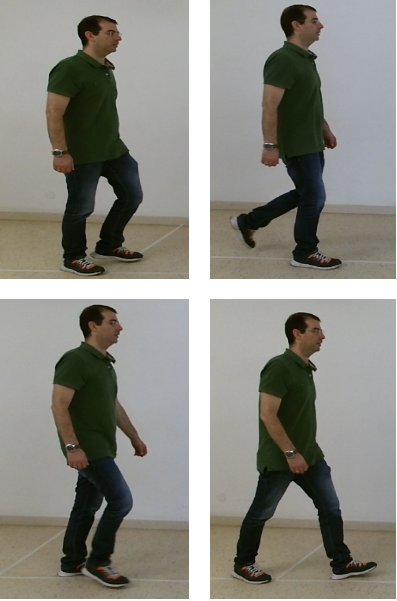
\includegraphics[width=\linewidth]{assets/gei-flow_a.png}
        \subcaption{RGB Image Sequence}
        \label{fig:silhouette-gei-image-processing_a}
    \end{minipage}
    \hfill
    \begin{minipage}{0.31\textwidth}
        \centering
        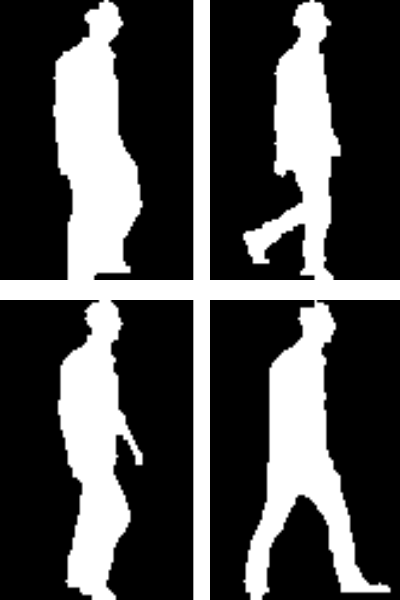
\includegraphics[width=\linewidth]{assets/gei-flow_b.png}
        \subcaption{Silhouette Sequence}
        \label{fig:silhouette-gei-image-processing_b}
    \end{minipage}
    \hfill
    \begin{minipage}{0.31\textwidth}
        \centering
        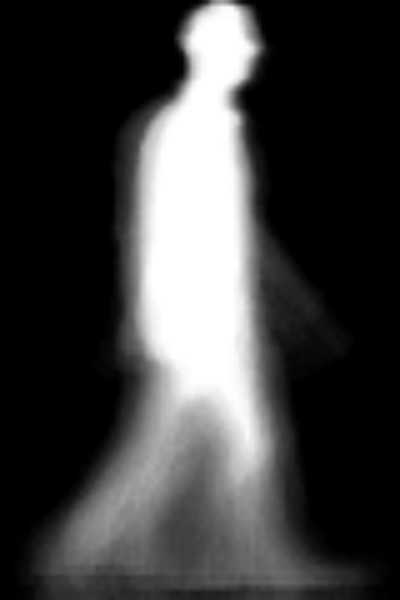
\includegraphics[width=\linewidth]{assets/gei-flow_c.png}
        \subcaption{\acf{gei}}
        \label{fig:silhouette-gei-image-processing_c}
    \end{minipage}
    \caption{Silhouette and \ac{gei} Image Processing Example}
    \caption*{\centering \textit{(Source: \cite{nunesGRIDDSGaitRecognition2019})}}
    \label{fig:silhouette-gei-image-processing}
\end{figure}


The current state-of-the-art shows \ac{dl}-based classification (see Section \ref{subsubsec:classification-techniques}) is optimal for \ac{gr} tasks, achieving Rank-1 accuracies (the percentage of times the top prediction is correct) north of 90\% on the CASIA-B dataset \parencite{gunersahanSurveyAppearancebasedApproaches2024}.
\ac{dl} reduces the need for manual feature engineering, enhancing classification efficiency.
This benefits accuracy, with traditional \ac{ml} methods (e.g., \ac{nn} or \ac{svm}) suffering a 10-20\% drop on more challenging datasets \parencite{shenComprehensiveSurveyDeep2023}.
In uncontrolled scenarios, environmental conditions, occlusion, and gait variations will have an impact on accuracy, regardless of classification approach.

Appearance-based \ac{gr} has in some cases been demonstrated using simpler methods that don't require training of an \ac{ml} model.
In a tutorial created for the 2016 International Conference on Pattern Recognition (ICPR), a \ac{gei}-based \ac{gr} system was demonstrated that calculated differences between pixels in a newly created (from real-time video) \ac{gei} image, against a database of historic \acs{gei} with assigned identities, finding the closest match based on the resulting statistical similarity scores \parencite{songDevelopfengGaitRecognition2024}.
Although suitable for demonstration and \ac{poc} purposes, simpler solutions forfeit many advantages achieved by \ac{ml}-based solutions, therefore their use in production environments may introduce reliability, usability, and security issues, instead of an improvement.

Overall, appearance-based \ac{gr} systems face some limitations, like reliance on view angle; if a classification model is trained on, or a set of \ac{gei} images is created, using lateral movement data, the camera used to capture subsequent gait cycles must be similarly positioned.
Anything obstructing a subject's figure (e.g., bags, baggy clothes, or external objects) will also have a greater impact on appearance-based \ac{gr} \parencite{hanIndividualRecognitionUsing2006}.
However, the resource efficiency compared to model-based solutions is advantageous; speed of identification and lesser resource requirements in a \ac{pacs}, contributing to a better user experience may influence choices for implementation \parencite{lingShapeClassificationUsing2007}.

\subsubsection{Classification Techniques}
\label{subsubsec:classification-techniques}

\ac{ai} and \ac{ml} have revolutionised the feature extraction and classification processes enhancing modern data analysis and biometric identification.
They automate traditionally manual tasks of identifying patterns and relationships in raw data to produce structured data, used for efficient classification or predictions based on input \parencite{bishopPatternRecognitionMachine2006}.
In the context of \ac{gr}, \ac{ai} and \ac{ml} can, and have been employed to extract information about gait patterns from appearance and model-based data, supporting the creation of models and classifiers capable of identifying individuals based on their walking style \parencite{ghilomRoleMachineLearning2024}.
Traditional \ac{ml} or \ac{dl} approaches can be used to achieve this, with \ac{dl} alternatively employing more complex algorithms to perform analysis at a more intricate level --- resulting in increased accuracy \parencite{shenComprehensiveSurveyDeep2023}.

\ac{nn} classification is a traditional method that categorises input based on the closest matching data point(s) --- vectors of features for an object --- in a 'neighbourhood' (imagine plotting points on a graph).
A common method of defining a neighbourhood is '$k$-\ac{nn}', where the closest $k$ number of data points contribute toward classification \parencite{faouziClassicMachineLearning2023}.
\ac{nn} has proven most suitable for smaller datasets, with performance degrading as the number of data points rises, as this demands computational effort.
For \ac{gr}, \ac{nn} could be used to compare static gait features, identifying subjects based on similarity (if any) to labelled historic data \parencite{myeducatorMyEducatorAdvantagesDisadvantages2024}.

\ac{pca} is a technique used in traditional classification workflows, it optimises, or 'reduces the dimensionality of' complex datasets, producing sets of independent components, while maintaining patterns important for classification.
\ac{pca} can be used to extract the most pertinent information from images in silhouette and \ac{gei}-based \ac{gr} systems, which is fed into algorithms like \ac{lda} or \acs{svm}, or used by simpler measures like $k$-\ac{nn} or cosine similarity.
\ac{lda} performs further optimisations, enhancing the separability of data points through abstraction, which are then classified by algorithms like $k$-\ac{nn}, cosine similarity, or \ac{pda} \parencite{hongyeGaitRecognitionBased2015}.
\acp{svm} perform optimisation by identifying the 'optimal hyperplane' --- decision boundary with the greatest margin between linearly separable (achieved by \ac{pca}) classes --- performing classification itself \parencite{kowalczykSVMUnderstandingMath2015}.

\ac{dl} has further improved the training and classification process by abstracting manual feature engineering steps (e.g., using a combination of \ac{pca}, \ac{lda}, and $k$-\ac{nn} for dataset optimisation and classification) producing end-to-end learning pipelines capable of identifying patterns in raw, unstructured data.
\acs{cnn} are a type of \ac{nn} and are the default \ac{dl} approach to many static image recognition tasks.
They automate the feature extraction, dimensionality reduction, and classification of spatial data, enabling unsupervised, iterative learning \parencite{bariKinectGaitNetKinectBasedGait2022}.
Many existing \ac{gr} systems using \acs{cnn} are appearance-based, performing classification on static (spatial) features of silhouette images or \acs{gei} \parencite{shenComprehensiveSurveyDeep2023}.

\acs{rnn}, another type of \ac{nn}, support analysis of temporal and sequential data. \acs{rnn} have been used in addition to \acs{cnn} for \ac{gr} purposes, enabling extraction of spatio-temporal information.
For example, given a dataset of sequential silhouettes, a \ac{cnn} would assess characteristics of individual images, whereas a \ac{rnn} would account for patterns occurring over time or throughout a sequence \parencite{hasanSilhouettebasedGaitRecognition2022}.

The automated framework implemented by \ac{nn}-based techniques allows for enhanced performance compared to traditional \ac{ml} techniques; \acs{nn} learn complex patterns from iterative, in-depth analysis of input \parencite{engatiConvolutionalNeuralNetwork2024}.

\subsection{Applications of Gait Recognition in Physical Access Control}
\label{subsec:applications-of-gait-recognition-in-physical-access-control}

Applications of biometric authentication in \ac{pacs} are not hard to come by, with 32\% of organisations surveyed in 2024 reporting their own implementations (see Section \ref{subsec:biometric-authentication-trends}).
Examples of \ac{gr}-based biometrics for \ac{pacs}, however, are not so common.
Many real-world examples of \ac{cv}-based gait analysis technologies are in the clinical or forensic fields (see Section \ref{subsec:gait-recognition-overview}) which although not contributing to access control, demonstrates the feasibility of extracting features from, and performing identification based on gait.

In October 2024, a European Union consortium launched a pilot project --- 'PopEye' --- to study how \ac{gr} technology can speed up identity checks at border crossings and reduce issues experienced with traditional types of biometrics (e.g., facial recognition, which is widely used at airports across Europe) when environmental conditions and/or appearance vary.
While not yet implemented, the project's success could lead to the adoption of Gait-based authentication technologies across European Union borders and in other environments, like workplaces \parencite{chrisburtPopEyeStrengthenEU2024}.

One of the rare production examples of a \ac{gr}-based authentication system for \ac{pacs} is Stepscan Secure.
This system does not use \ac{cv}, instead assessing walking style using under-floor pressure sensors. The product is advertised as a more 'secure alternative to traditional \ac{pacs} \ac{mfa}' methods \parencite{stepscanGaitAuthenticationSecurity2020}.
The organisation behind the technology started out producing medical gait assessment systems and appear to have identified the gap in the market for an unobtrusive, transparent authentication solution.
It is not clear how varying types of footwear may affect the system's effectiveness in identifying individuals but may have a similar effect to occlusion in \ac{cv}-based solutions.


\subsection{Perceived Public Opinion (via Survey)}
\label{subsec:perceived-public-opinion-via-survey}

To gain insight into the public perception of the concept of \ac{gr}-based authentication, a questionnaire was distributed to members of the public, requesting they rate their perceived security, comfort, and willingness to adopt \ac{gr}-based identification technologies. A view of the questionnaire can be seen in Appendix \ref{app:public-opinion-survey}, with twenty-one (21) responses collected from people aged between 18 and 34.

\paragraph{Comfort and Acceptability} Most respondents fell in the middle range, specifying they were 'Somewhat Comfortable' or 'Somewhat Uncomfortable' with the concept of \ac{gr}. Verfy few respondents expressed strong feelings in either direction, with only one respondent being 'Very Comfortable' and one being 'Very Uncomfortable', stating: 'I'm not comfortable with giving up my personally identifiable data for the simple purpose of access control'. A majority of respondents rated \ac{gr};s security level as moderate, specifying 'Neutral' to 'Somewhat Secure'.

\paragraph{Perceived Security} Respondents generally perceived \ac{gr} as less secure than fingerprint or facial recognition, with most rating the security level between 2 and 4 on a 5-point scale. However, opinions on traditional methods like \ac{rfid} cards and \ac{pin} codes were often perceived as less secure than biometrics overall.

\paragraph{Authentication Preferences} Only two respondents selected 'passive authentication' as their preferred method of authentication going forward, with the majority preferring traditional methods like \ac{rfid} cards and \ac{pin} codes, or more established biometric methods. The respondents that did select \ac{gr} as their preferences also cited convenience as a high priority, with one also stating: 'Sometimes my RFID Chip doesn't work on the first try and i have to try again'.

\paragraph{Concerns and Requirements} In order to increase comfort with biometric systems including \ac{gr}, respondents prioritized:

\begin{itemize}
    \item Clear information about data storage
    \item Assurance that biometric data remains on-site (not cloud-stored)
    \item Transparent privacy policies
    \item Option to delete data when leaving an organization
    \item Regular system audits
    \item Alternative authentication methods being available
\end{itemize}

\paragraph{Demographics} The survey primarily captured younger adults, with submission ages ranging from 18 to 34. No clear correlation was observed between demographic factors and attitude toward \ac{gr}. However, one respondent noted concerns with bias in facial recognition, as they had experienced issues due to a combination of poor lighting and a darker skin complexion in the past.

\paragraph{Interest in Enrollment} When asked about willingness to participate in \ac{gr} enrollment, 4 respondents indicated "Yes", 3 respondents indicated "No", and the remaining respondents were "Unsure". This suggests moderate openness to the technology if properly implemented and proven to be effective.

Overall, these insights show that although there is some interest in \ac{gr}, there are also significant concerns regarding privacy, data storage, and percieved security levels when compared to alternative biometric methods. If implemented, a \ac{gr}-based system would need to have proved accuracy and reliability to gain widespread acceptance.


\subsection{Review Summary}
\label{subsec:review-summary}

Decades-old technologies remain dominant in the \ac{pacs} market despite known vulnerabilities and a user experience issues.
A level of complacency in physical security is demonstrated by organisations not prioritising moving to more secure solutions.
It can be argued that traditional methods are a burden on users, requiring physical tokens and a diversion of attention.
This creates opportunity for more convenient, less obtrusive alternatives --- \textit{what if authentication for \acf{pacs} could be invisible?}

As discussed in Section \ref{sec:gait-recognition-for-physical-access-control}, biometric-based authentication solutions have improved both security and usability by using inherent credentials that are more difficult to compromise and reduce user encumberment.
Of the most common solutions, facial recognition stands out by making it possible to determine identity from a distance, reducing the time sink of repeated interaction with access control interfaces.
However, its reliability can be influenced by factors like resolution, environment, face coverings, and darker skin tones.
Emerging biometrics, like \ac{gr}, serve as promising solutions to these issues. By assessing walking patterns and body movement to verify identity, \ac{gr} achieves similar advantages to facial recognition while combatting many weaknesses by evaluating more than just facial features.

Although thoroughly researched, \ac{gr} --- especially \ac{cv}-based --- has yet to see widespread adoption in \acs{pacs}. Feedback from the public (see Section \ref{subsec:perceived-public-opinion-via-survey}) shows that there is a moderate willingness to adopt \ac{gr} if it can be proven to be secure and reliable, guaranteeing privacy and data security.
This provides an opportunity to advance verification and authentication, popularising forms of authentication that eliminate the need for physical tokens and operate 'transparently', using robust and hard-to-compromise credentials, can improve both \ac{pacs} security and usability.

The following chapter --- 'New Ideas' --- proposes a \ac{gr}-based authentication system as an alternative to traditional token-based and biometric authentication methods.
It addresses concerns raised in this chapter in relation to security, usability, and ethics, discussing how the it may help make improvements to these areas.